\documentclass[11pt]{article}
\usepackage{graphicx}
\graphicspath{{images/}}
\usepackage{listings}
\usepackage{color}
\usepackage[utf8]{inputenc}
\usepackage{float}
\usepackage{siunitx}
\usepackage{tabto}
\usepackage{caption}
\usepackage{multirow}
\usepackage{pdfpages}
\usepackage[titletoc,toc]{appendix}
\usepackage{fancyhdr}
\usepackage{amsmath}
\usepackage[hidelinks]{hyperref}


\fancyhf{}
\setlength{\headheight}{0pt}
\renewcommand{\headrulewidth}{0pt}
\pagestyle{fancy}
\pagenumbering{gobble}

\definecolor{comment}{rgb}{0,0.6,0}
\definecolor{code}{rgb}{0.58,0,0.82}

\lstset{
	backgroundcolor=\color{white},
	commentstyle=\color{comment},
	frame=tb,
	keywordstyle=\color{blue},
	stringstyle=\color{code},
	language=C,
	basicstyle={\small\ttfamily}
}
\title{\textbf{HC-05 Bluetooth extension Design}}
\author{Virgile Neu}
\date{\today \\ version 2.6}
\begin{document}
\maketitle
    \begin{figure}
        \center
        
\includegraphics[scale=0.9]{EPFL-Logo-CMJN.eps}
    \end{figure}
    \newpage
    
\tableofcontents

\newpage

\pagenumbering{arabic}
\setcounter{page}{1}
\lfoot{EPFL}
\cfoot{Virgile Neu}
\rfoot{\thepage}

\section{Introduction}

The HC-05 chip is a Bluetooth module with a AT command mode. It can be used as a Bluetooth master or slave, with the possibility of connecting to the previous connection automatically at start-up. It can also boot into the AT Command mode and set all parameters, list the available peripherals and connect to one.\\
It has 5 pins of interest plus \texttt{VCC} and \texttt{GND} : \texttt{EN}, \texttt{STATE}, \texttt{Rx}, \texttt{Tx} and the pin34 (\texttt{ATSel}). The picture \ref{hc05} below show the hc05 board with it's connectivity.
\begin{figure}[H]
        \makebox[\textwidth][c]{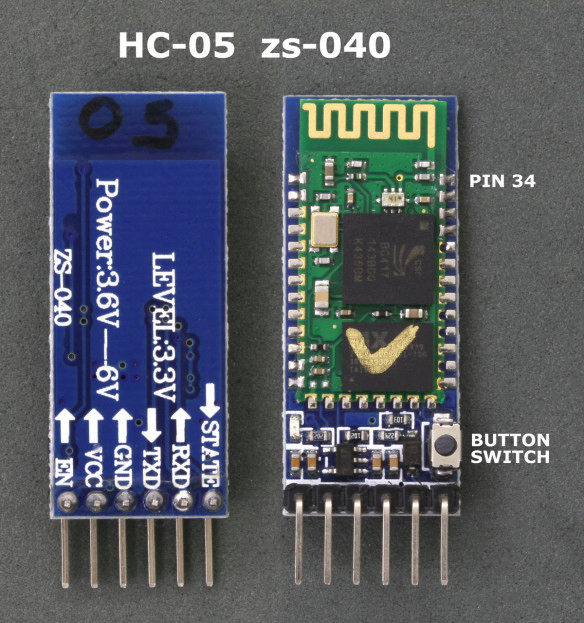
\includegraphics[width=0.8\textwidth,keepaspectratio]{hc05.png}}
        \caption{The hc05 module.}
        \label{hc05}
\end{figure}

The goal is to make available this Bluetooth module to use on the FPGA and to make it easily usable. Figure \ref{uses_flowchart} depicts how to use it from the CPU point of view.

\begin{figure}[H]
        \makebox[\textwidth][c]{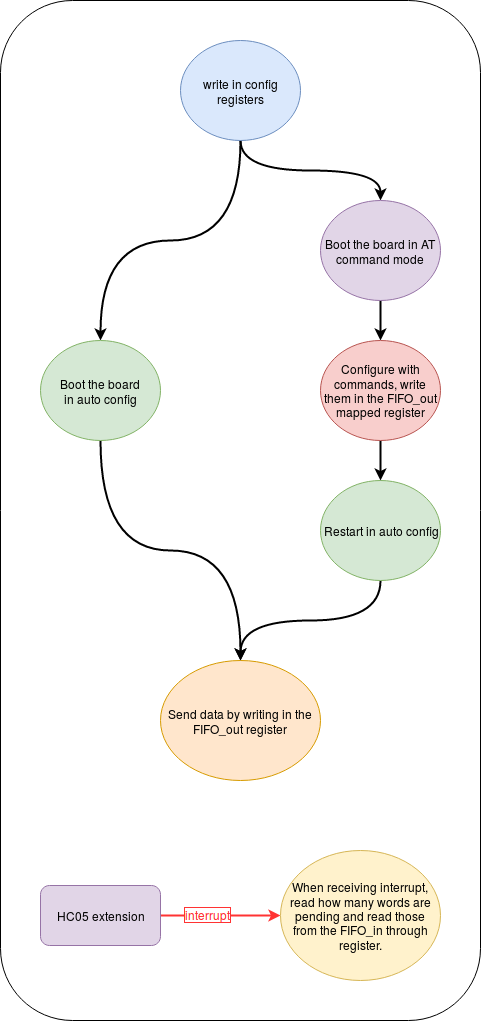
\includegraphics[width=0.9\textwidth,height=0.9\textheight,keepaspectratio]{uses_flowchart.png}}
        \caption{Uses flowchart seen by the CPU.}
        \label{uses_flowchart}
\end{figure}
\newpage
\section{Parameters}

\subsection{Default configuration}
\begin{itemize}
    \item Device type : 0
    \item Inquire code : 0x009e8b33
    \item Module work mode : Slave Mode
    \item Connection mode : Connect to the BT device specified
    \item Baud rate : 9600 bits/s
    \item Stop bit : 1 bit
    \item Parity bit : None
    \item Passkey : "1234"
    \item Device name : "HC-05"
\end{itemize}

\subsection{Serial Parameters}
The HC05 supports all these parameters for the serial communication on the UART ports :
\subsubsection{Baud rates}
\begin{itemize}
    \item 4800 bits/s
    \item 9600 bits/s
    \item 19200 bits/s
    \item 38400 bits/s
    \item 57600 bits/s
    \item 115200 bits/s
    \item 230400 bits/s
    \item 460800 bits/s
    \item 921600 bits/s
    \item 1382400 bits/s
\end{itemize}

\subsubsection{Stop bit}
\begin{itemize}
    \item 1 bit
    \item 2 bit
\end{itemize}

\subsubsection{Parity bit}
\begin{itemize}
    \item None
    \item Odd parity
    \item Event parity
\end{itemize}

The UART works as described on figure \ref{UART_data_transfert}. It starts with the start bit, always '0', then comes the data (here 8 bits), least significant bit first, then the parity bit (if set), and then 1 or 2 stop bit, always '1'.
\begin{figure}[H]
        \makebox[\textwidth][c]{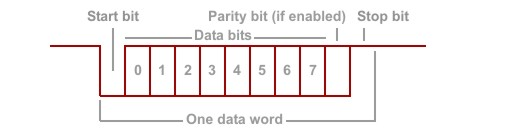
\includegraphics[width=\textwidth,height=\textheight,keepaspectratio]{uart_data.jpg}}
        \caption{UART data transfert.}
        \label{UART_data_transfert}
\end{figure}
\subsection{Connection mode}
The HC05 has three Bluetooth connection modes :
\begin{itemize}
    \item Connect to specified address
    \item Connect to any address
    \item Slave-Loop
\end{itemize}

\section{Design Choices}
Here I will show how the extension will look like, see figure \ref{high_level}. It will consist of Four parts:
\begin{itemize}
    \item Registers, to store configuration, status and other things,
    \item A FIFO\_OUT to send data from the CPU to the UART custom interface,
    \item A FIFO\_IN to receive data from the HC05,
    \item A custom UART interface to communicate to the HC05.
\end{itemize}
\begin{figure}[H]
        \makebox[\textwidth][c]{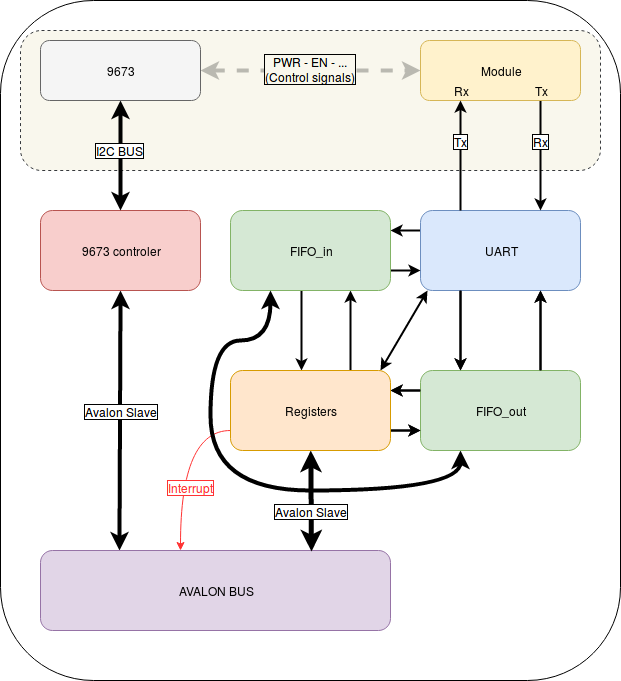
\includegraphics[width=\textwidth, height=\textheight,keepaspectratio]{highlevel.png}}
        \caption{High level block diagram of the HC05 extension.}
        \label{high_level}
\end{figure}

\subsection{Registers}
The registers will have height registers :
\begin{itemize}
    \item A control register \texttt{CTRL},
    \item A status register \texttt{STATUS},
    \item A register for the \texttt{UART waiting cycles} (depends on the UART rate),
    \item The \texttt{FIFO\_out\_data} register,
    \item The \texttt{FIFO\_out\_free\_space} register,
    \item The \texttt{FIFO\_in\_data} register,
    \item The \texttt{FIFO\_in\_pending\_data} register.
    \item The \texttt{reset\_FIFO} register.
\end{itemize}
Here is the register map in table \ref{reg_map} below.
\texttt{
\captionof{table}{Register map of the Registers component.}
\label{reg_map}
\centerline{
\begin{tabular}{|l|l|c|c|c|c|c|c|c|c|c|c|c|}
\hline
\# & addr & 31..8 & 7 & 6 & 5 & 4 & 3 & 2 & 1 & 0 & R/W\\
\hline
0 & 0x00 & \multicolumn{3}{c|}{Unused} & \multicolumn{3}{c|}{\texttt{UART\_CTRL}} & \multicolumn{2}{c|}{\texttt{I\_ENABLE}} & \texttt{\texttt{UART\_ON}} & R/W\\
\hline
1 & 0x04 & \multicolumn{7}{c|}{Unused} & \multicolumn{2}{c|}{\texttt{i\_pending}} & R/W\\
\hline
2 & 0x08 & \multicolumn{9}{c|}{\texttt{UART\_wait\_cycles}} & R/W\\
\hline
3 & 0x0C & ignored & \multicolumn{8}{c|}{\texttt{FIFO\_out\_data}} & W\\
\hline
4 & 0x10 & \multicolumn{9}{c|}{\texttt{FIFO\_out\_free\_space}} & R\\
\hline
5 & 0x14 & zeros & \multicolumn{8}{c|}{\texttt{FIFO\_in\_data}} & R\\
\hline
6 & 0x18 & \multicolumn{9}{c|}{\texttt{FIFO\_in\_pending\_data}} & R\\
\hline
7 & 0x1C & \multicolumn{7}{c|}{Unused} & \texttt{reset\_out} & \texttt{reset\_in} & W\\
\hline
\end{tabular}}
\begin{center}
\begin{tabular}{|c|c|c|}
\hline
\multicolumn{3}{|c|}{UART\_CTRL}\\
\hline
5 & 4 & 3\\
\hline
\multicolumn{2}{|c|}{\texttt{parity\_bit}} & \texttt{stop\_bit}\\
\hline
\end{tabular}
\begin{tabular}{|c|c|}
\hline
\multicolumn{2}{|c|}{I\_ENABLE}\\
\hline
2 & 1\\
\hline
\texttt{i\_dropped} & \texttt{i\_received}\\
\hline
\end{tabular}
\end{center}
}
The role of each bit is described below :
\begin{itemize}
    \item 0x00 :
    \begin{itemize}
        \item \texttt{UART\_ON} : Specifies if the UART will capture or send data or if it will stay off.
        \item \texttt{i\_received} : Specifies if the device can send interrupts request when receiving data from the HC05.
        \item \texttt{i\_dropped} : Specifies if the device can send interrupts request when some data is dropped.
        \item \texttt{stop\_bit} : Specifies the number of stop bit, '0' for 1, '1' for 2.
        \item \texttt{parity\_bit} : Specifies the parity bit, "00" for None, "10" for Even and "11" for Odd.
    \end{itemize}
    \item 0x04 : 
    \begin{itemize}
        \item \texttt{i\_pending} : Tells if there is an interrupt waiting to be served by the CPU. The CPU must clear it by software when serving the interrupt. Bit 0 is for \texttt{i\_received}, bit 1 is for \texttt{i\_dropped}. Writing '1' to any of the two bits has no effect.
    \end{itemize}
    \item 0x08 : \texttt{UART\_wait\_cycles} : Specifies to the UART how many cycles it should wait before capturing the values during the transfert. The values to put are described in the table \ref{UART_wait_cycles} below for a 50MHz clock. 
    \item 0x0C : \texttt{FIFO\_out\_data} : Address to write to send data to the HC05 through the \texttt{FIFO\_out}. The write must has the byte\_enable signal equal to "0001".
    \item 0x10 : \texttt{FIFO\_out\_free\_space} : Number of free words (10 bits) in the \texttt{FIFO\_out}. 
    \item 0x14 : \texttt{FIFO\_in\_data} : Address to read to receive data from the HC05 through the \texttt{FIFO\_in}. 
    \item 0x18 : \texttt{FIFO\_out\_free\_space} : Number of waiting words (11 bits) in the \texttt{FIFO\_in}. 
    \item 0x1C :
    \begin{itemize}
        \item \texttt{reset\_in} : Write only bit to clear the \texttt{FIFO\_in}.
        \item \texttt{reset\_out} : Write only bit to clear the \texttt{FIFO\_out}.
    \end{itemize}
\end{itemize}
\newpage
The value to put in the \texttt{UART\_wait\_cycles} registers depend on the desired UART baud rate, and is computed with the following formula.
\begin{align*}
wait\_cycles &= \frac{time\_per\_bit}{time\_per\_cycles}\\
&= \frac{\frac{1}{baud\_rate}}{clk\_period} \\
&= \frac{clk\_freq}{baud\_rate}
\intertext{For 4800 bits/s of baud rate we have.}
wait\_cycles &= \frac{clk\_freq}{baud\_rate}\\
&= \frac{50\cdot 10^{6}}{4800} = 10416.667 \quad clk\_cycles
\end{align*}
The rounding doesn't matter.
\captionof{table}{\texttt{UART\_wait\_cycles} values for a given UART.}
\label{UART_wait_cycles}
\begin{center}
\begin{tabular}{|l|r|}
\hline
UART\_Rate & wait\_cycles value (decimal)\\
\hline
4800 bits/s & 10416 clk\_cycles\\
\hline
9600 bits/s & 5207 clk\_cycles\\
\hline
19200 bits/s & 2604 clk\_cycles\\
\hline
38400 bits/s & 1302 clk\_cycles\\
\hline
57600 bits/s & 868 clk\_cycles\\
\hline
115200 bits/s & 434 clk\_cycles\\
\hline
230400 bits/s & 217 clk\_cycles\\
\hline
460800 bits/s & 109 clk\_cycles\\
\hline
921600 bits/s & 54 clk\_cycles\\
\hline
1382400 bits/s & 36 clk\_cycles\\
\hline
\end{tabular}
\end{center}

When using autoconnect, the device will simply boot with the last configuration used. When using AT command mode, the CPU will have to initiate itself the connection, and can change modes or settings.
\\\\
The ports of the Registers component are described on figure \ref{reg_ports} below.
\begin{figure}[H]
        \makebox[\textwidth][c]{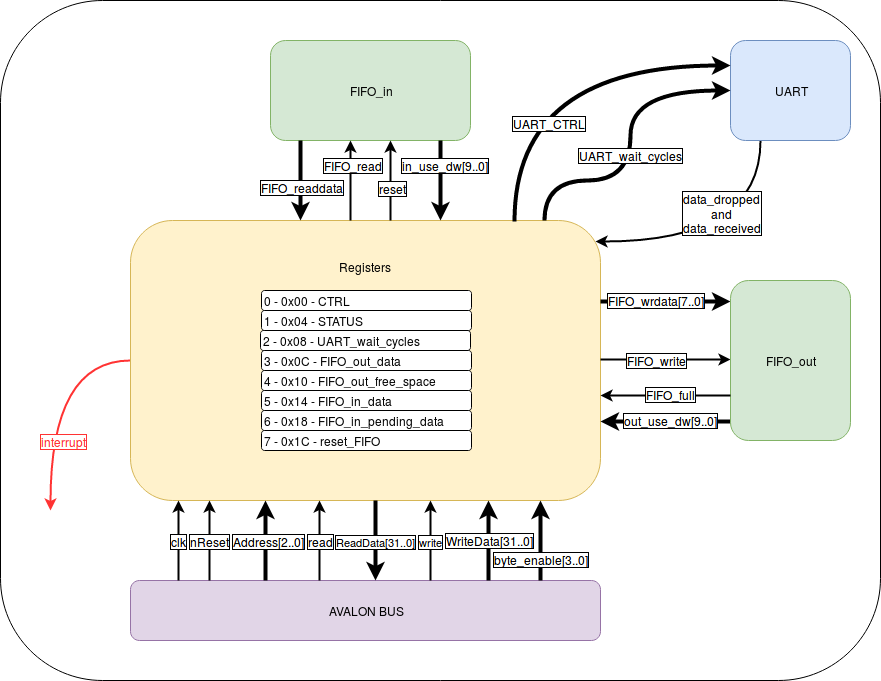
\includegraphics[width=\textwidth, height=\textheight,keepaspectratio]{registers_ports.png}}
        \caption{Ports description of the Registers component.}
        \label{reg_ports}
\end{figure}

\subsection{FIFO\_out}
For the \texttt{FIFO\_out} we will use the FIFO available in the IP catalogue of Quartus with the following configurations :
\begin{itemize}
    \item Width = 8 bits,
    \item Depth = 1024 (biggest size with only one M10k element),
    \item control signals : \begin{itemize}
        \item use\_dw[] (10 bits),
        \item empty,
        \item asynchronous clear; \end{itemize}
    \item Show ahead FIFO mode,
    \item Auto memory block type,
    \item No optimisation or circuitry protection.
\end{itemize}

The ports of the \texttt{FIFO\_out} component are described on figure \ref{fifo_out_ports}.
\begin{figure}[H]
        \makebox[\textwidth][c]{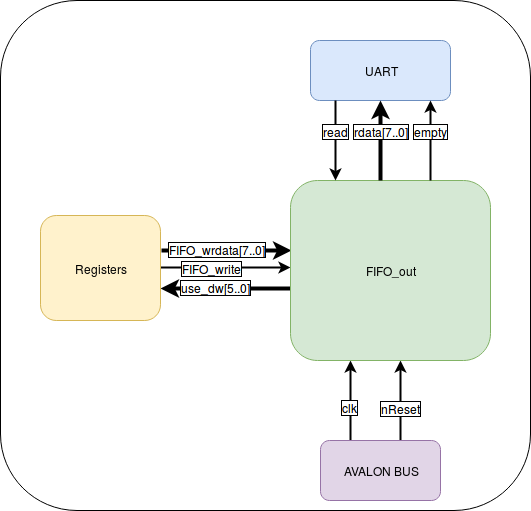
\includegraphics[width=\textwidth, height=\textheight,keepaspectratio]{FIFO_out_ports.png}}
        \caption{Ports description of the \texttt{FIFO\_out} component.}
        \label{fifo_out_ports}
\end{figure}
\pagebreak
\subsection{FIFO\_in}
For the \texttt{FIFO\_in} we will also use the FIFO available in the IP catalogue of Quartus with almost the same configurations :
\begin{itemize}
    \item Width = 8 bits,
    \item Depth = 1024 (biggest size with only one M10k element),
    \item control signals : \begin{itemize}
        \item use\_dw[] (10 bits),
        \item full,
        \item asynchronous clear; \end{itemize}
    \item Normal synchronous FIFO mode,
    \item Auto memory block type,
    \item No optimisation or circuitry protection.
\end{itemize}

The ports of the \texttt{FIFO\_in} component are described on figure \ref{fifo_in_ports}.
\begin{figure}[H]
        \makebox[\textwidth][c]{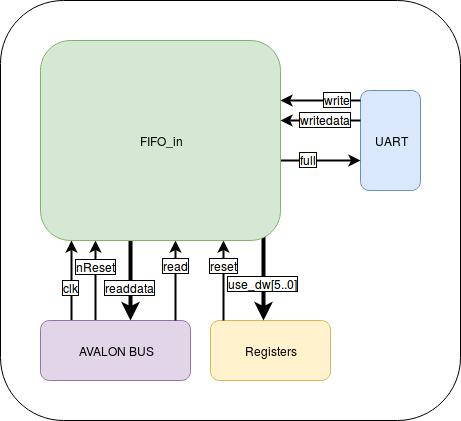
\includegraphics[width=\textwidth, height=\textheight,keepaspectratio]{FIFO_in_ports.png}}
        \caption{Ports description of the \texttt{FIFO\_in} component.}
        \label{fifo_in_ports}
\end{figure}

\subsection{UART}
The UART will be the part communicating with the HC05 module. It will send whenever it can while the \texttt{FIFO\_out} isn't empty, and whenever it receives information, it will recompose the words, perform the parity check (if set) and send the correct words to the \texttt{FIFO\_in}.
\\
The ports of the UART component are described on figure \ref{uart_ports}.
\begin{figure}[H]
        \makebox[\textwidth][c]{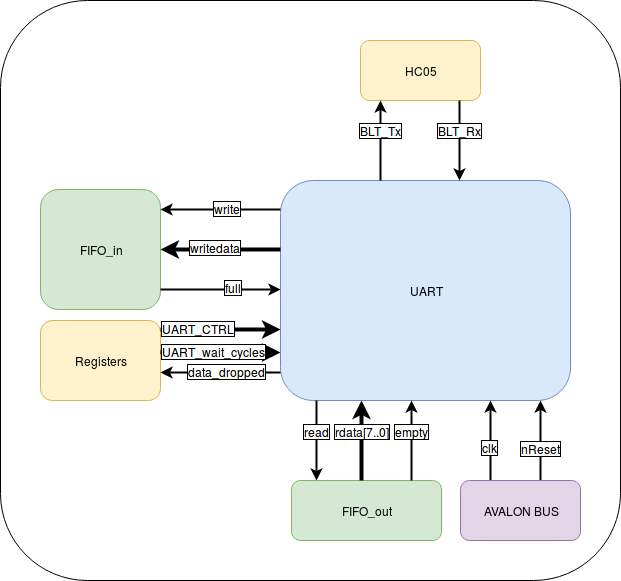
\includegraphics[width=\textwidth, height=\textheight,keepaspectratio]{UART_ports.png}}
        \caption{Ports description of the UART component.}
        \label{uart_ports}
\end{figure}

\section{Pinout}
The external connectivity of the device is described on table \ref{pinout}.
\begin{center}
\captionof{table}{Pinout table of the device.}
\label{pinout}
\begin{tabular}{|c|c|}
\hline
signal name & connectivity\\
\hline
\texttt{BLT\_RxD} & \texttt{GPIO\_1 8 -- FPGA PIN\_AE22}\\
\hline
\texttt{BLT\_TxD} & \texttt{GPIO\_1 6 -- FPGA PIN\_AH24}\\
\hline
\texttt{BLT\_State} & \multirow{3}{*}{\texttt{PCA9673} via Avalon Bus}\\
\cline{1-1}
\texttt{BLT\_EN} &\\
\cline{1-1}
\texttt{BLT\_ATSel} &\\
\hline
\end{tabular}
\end{center}

\section{States Machines}
This section describes the several states machines used in the extension.
\subsection{UART}
\subsubsection{Transmitting State Machine}
The figure \ref{UART_transmit_SM} below describe the state machine used for transmitting data. It consists of 5 states : WAITING, START, SENDING, PARITY and STOP states. It starts at the WAITING states, and wait for data to be available in the \texttt{FIFO\_out}. Once data is available, it issue a read to the \texttt{FIFO\_out} and go to the start states. During the start state, it outputs the '0' value, as specified in the UART protocol, and store the data from the \texttt{FIFO\_out\_readdata} during the first cycle in this state. Once it has waited enough, it goes to sending. During sending state, it will send bit after bit, every time waiting the good amount of time. Oncei all the 8 bit of data are sent, it will either go to STOP if the parity is disabled (\texttt{parity\_bit} = "00") or to PARITY if it is enable. In the PARITY state, it will output the parity value (odd or even) for the right amount of time, and then go to the STOP state. In the STOP state, it will output 1 or 2 bit at '1', depending on the settings of the \texttt{stop\_bit}, and then go to the WAITING state, ready to transfer again.
\begin{figure}[H]
        \center
        \makebox[\textwidth][c]{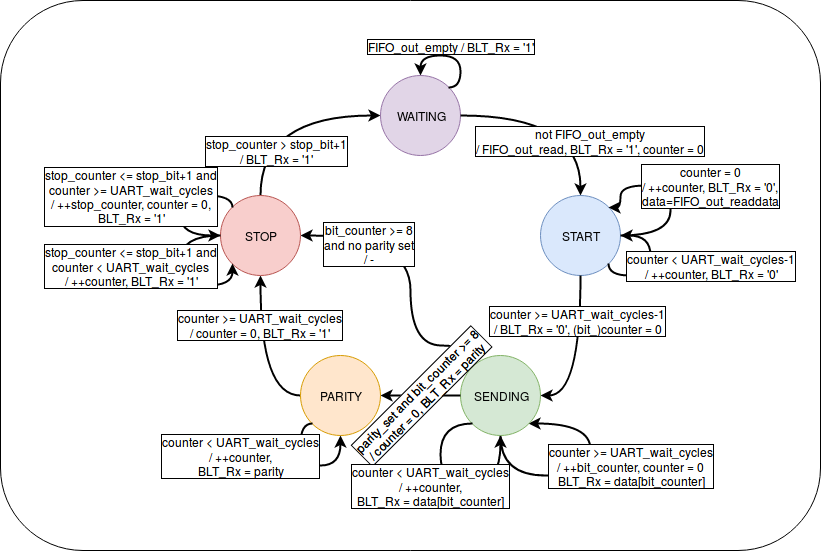
\includegraphics[width=\textwidth, height=\textheight,keepaspectratio]{UART_transmit_SM.png}}
        \caption{State machine used for sending one word (8 bits) to the HC05.}
        \label{UART_transmit_SM}
\end{figure}
\subsubsection{Receiving State Machine}
The figure \ref{UART_receive_SM} below describe the state machine used for receiving data. It has 4 states : WAITING, START, RECEIVING and PARITY. It starts at the WAITING states, and wait until the BLT\_Tx is '0' (start bit). Then we wait for half the cycles to wait in the START state in order to capture each bit in correctly and not just when they are supposed to go up (in order to avoid wrong bits), continuously checking that the start bit is still on (BLT\_Tx = '0'). Then we go to the RECEIVING state, where we wait for a full wait before capturing each bit. There is a transition back to the WAITING state with a big condition, it is to catch an error in the start bit during the first half of the first wait round. Once we received all the bits, we either go to the parity check in the PARITY state if enable or directly to the WAITING state and writing the data to the \texttt{FIFO\_in} if it is not full. If we go to the PARITY state, we check if the parity of the data we received is correct, and if it is we write it to the \texttt{FIFO\_in} if it is not full, and else we discard it. Then we go back to WAITING.
\begin{figure}[H]
        \makebox[\textwidth][c]{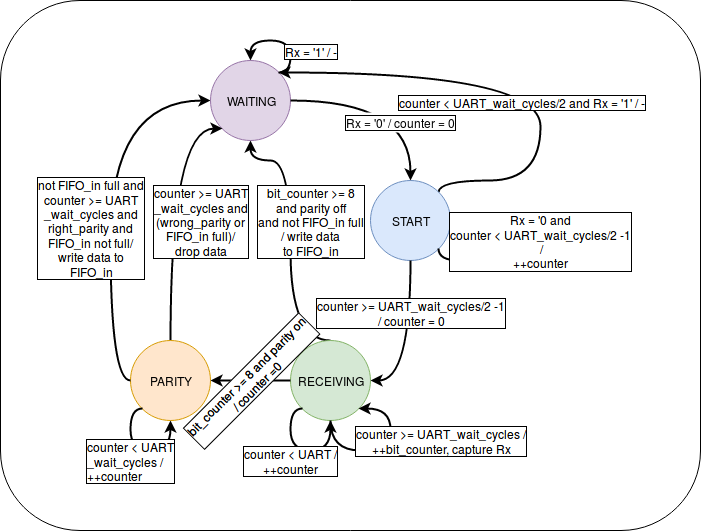
\includegraphics[width=\textwidth, height=\textheight,keepaspectratio]{UART_receive_SM.png}}
        \caption{State machine used for receiving one word (8 bits) from the HC05.}
        \label{UART_receive_SM}
\end{figure}
\newpage
\section{Power consumption}
The HC05 device has a different power consumption depending on its mode and if it is transmitting or receiving data. The values have been measured with a constant 5V input for all the baud rates and it appears that it has no effect on the power consumption. The results can be found on the table \ref{power_consumption} below.

\begin{center}
\captionof{table}{Power consumption of the HC05 device}
\label{power_consumption}
\begin{tabular}{|c|c|c|l|}
\hline
Mode & I(mA) & P(mW) & Notes\\
\hline
Not enable & 5 & 20 & \\
\hline
AT command mode & 15 & 65 & Receiving or not has no impact\\
\hline
Slave mode not connected & 40 & 200 & \\
\hline
Slave mode connected & 20 & 100 & Spikes at 60mA/300mW every 130ms\\
\hline
Receiving data & 60-80 & 300-400 & \multirow{2}{*}{Not constant, spikes every 0.5ms}\\
\cline{1-3}
Transmitting data & 60-80 & 300-400 & \\
\hline
\end{tabular}
\end{center}

\section{Bluetooth transfer rate}
The data transfer rate between the HC05 and another bluetooth device have been measured. The baud rate has a significant impact on it, especially at low rates. The results are presented below on table \ref{throughput_table} and figure \ref{throughput_fig}.\\
The data throughput is almost constant when higher than 57600 b/s of baud rate, and the only thing changing is the packet size when above 460800 b/s.
\begin{center}
\captionof{table}{Throughput between the HC05 and another bluetooth device}
\label{throughput_table}
\begin{tabular}{|c|c|c|}
\hline
Baud rate & Throughput(b/s) & Packet size (b)\\
\hline
4800 & 3800 & 35 \\
\hline
9600 & 8550 & 70 \\
\hline
19200 & 15100 & 130 \\
\hline
38400 & 33000 & 250 \\
\hline
57600 & 41300 & 250 \\
\hline
115200 & 91500 & 350 \\
\hline
230400 & 130000 & 650 \\
\hline
460800 & 140000 & 650 \\
\hline
921600 & 168500 & 730 \\
\hline
1382400 & 165000 & 890\\
\hline
\end{tabular}
\end{center}
\begin{figure}[H]
\center
\makebox[\textwidth][c]{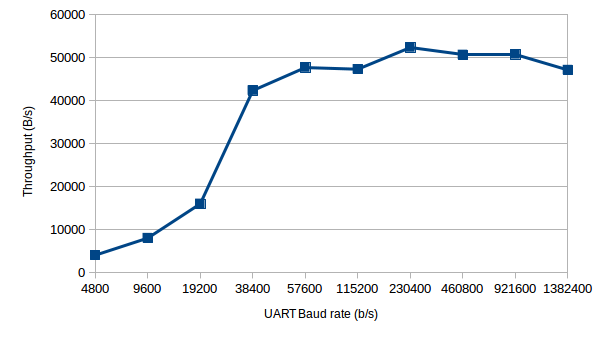
\includegraphics[width=\textwidth, height=\textheight,keepaspectratio]{throughput.png}}
\caption{Throughput of the HC05 depending on the Baud rates.}
\label{throughput_fig}
\end{figure}

\section{Bluetooth protocol}
The HC05 uses the L2CAP bluetooth protocol to transmit data over a bluetooth connection. This protocol supports segmentation and reassembly of packets, with a max packet payload of 64 kB. It also supports flow control and retransmission of packets. In theory, this protocol could also be used to do group-oriented communication, with different communication channels possible, but it is not used by the HC05.

\newpage
\begin{appendices}

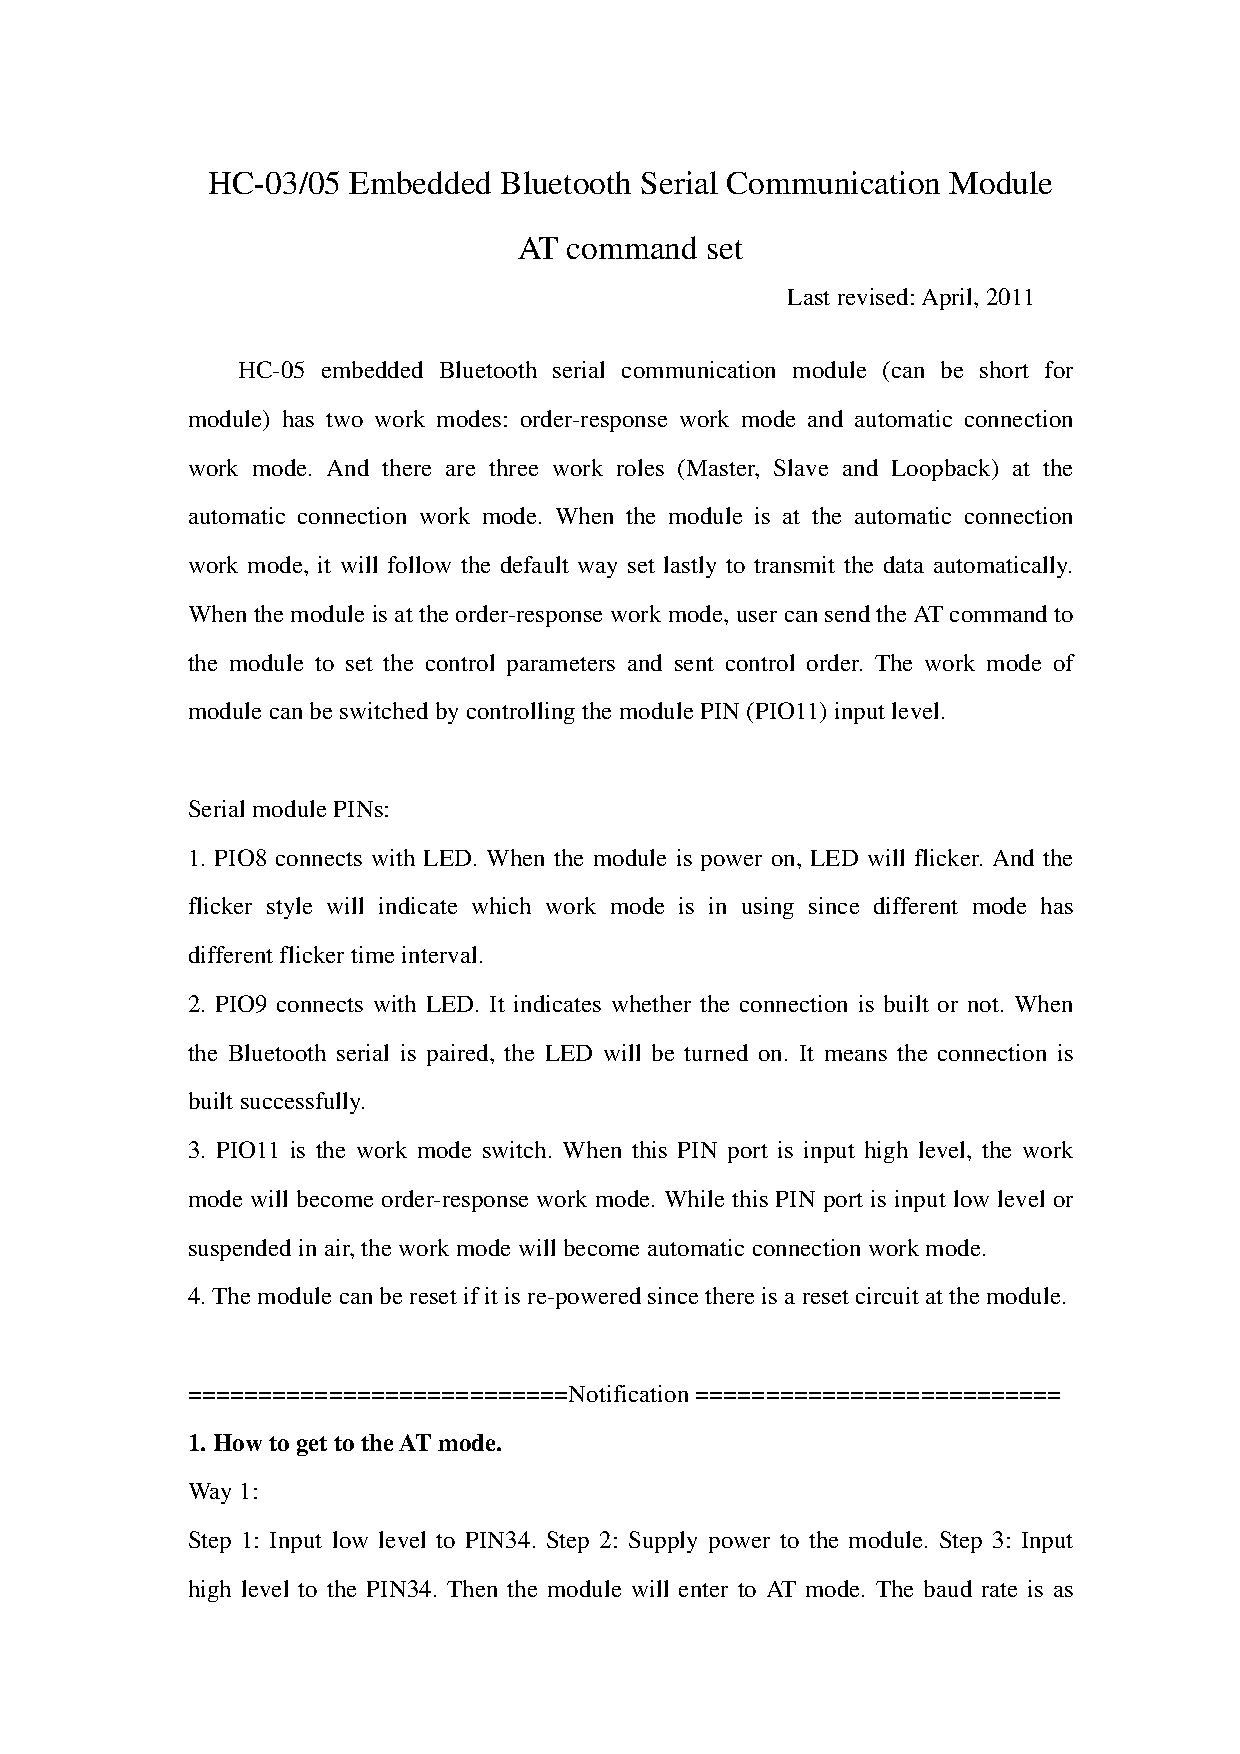
\includepdf[pages={1}, scale=.82, pagecommand=\section{AT Command Set}]{at_commands.pdf}
\includepdf[pages={2-}, scale=.82, pagecommand={}]{at_commands.pdf}

\end{appendices}

\end{document}
